\documentclass[crop=false, class=book]{standalone}

\usepackage{lipsum}
\usepackage{subfig}

\begin{document}
	
	
	\section{ALLPATHS-LG}
	\textit{ALLPATHS-LG} è un programma che permette di eseguire il sequenziamento di un genoma tramite de novo assembly di shotgun, e che calcola implicitamente la dimensione totale del genoma. Esso si basa sul programma \textit{ALLPATHS} \cite{butler2008allpaths,maccallum2009allpaths2} sviluppato precedentemente, e rispetto al suo predecessore permette l'assembly di genomi di dimensioni maggiori e con copertura minore, di gestire sequenze ripetitive, di correggere errori di lettura e di utilizzare in modo più efficiente le risorse disponibili durante il sequenziamento \cite{gnerre2011high}. 
	
	
	\subsection{Algoritmo}
	L'algoritmo del programma si basa sul precedente software ALLPATHS \cite{butler2008allpaths}. Dato un numero minimo $k$ di basi che si sovrappongono nelle letture shotgun, si definisce \textit{branch} una sequenza di $k$ basi (k-mer) che compare in due o più letture diverse, e la cui base successiva o precedente è diversa in ogni lettura. Spezzando il genoma in corrispondenza di ciascun branch, esso viene scomposto in un insieme di sequenze, dette \textit{unipath}. Tali sequenze vengono create a partire dalle letture shotgun di input non allineate. 
	
	\paragraph{Formazione dei k-mer path}
	Inizialmente negli shotgun viene corretto il maggior numero di errori di lettura, e vengono poi riconosciuti tutti i k-mer di lunghezza $k$. In ogni sequenza, ciascun k-mer viene numerato con un numero intero unico; a k-mer già trovati viene assegnato lo stesso valore. In questo modo ciascuna lettura potrà essere espressa come una sequenza di numeri interi, ognuno dei quali rappresenta un k-mer. 
	
	I numeri della sequenza vengono poi raggruppati in intervalli, in modo da formare i \textit{k-mer path}; essi associano ciascun intervallo al k-mer path a cui esso appartiene, permettendo una facile ricerca di tutte le sequenze che condividono un certo k-mer e semplificando quindi l'assembly delle letture shotgun. Si veda la figura~\vref{fig:allpathsnumbering} per un esempio su come avviene la numerazione dei k-mer e la creazione dei k-mer path.
	Le letture così tradotte costituiscono il database in cui è possibile effettuare ricerche per la costruzione degli unipath.
	
	\begin{figure}
		\centering
		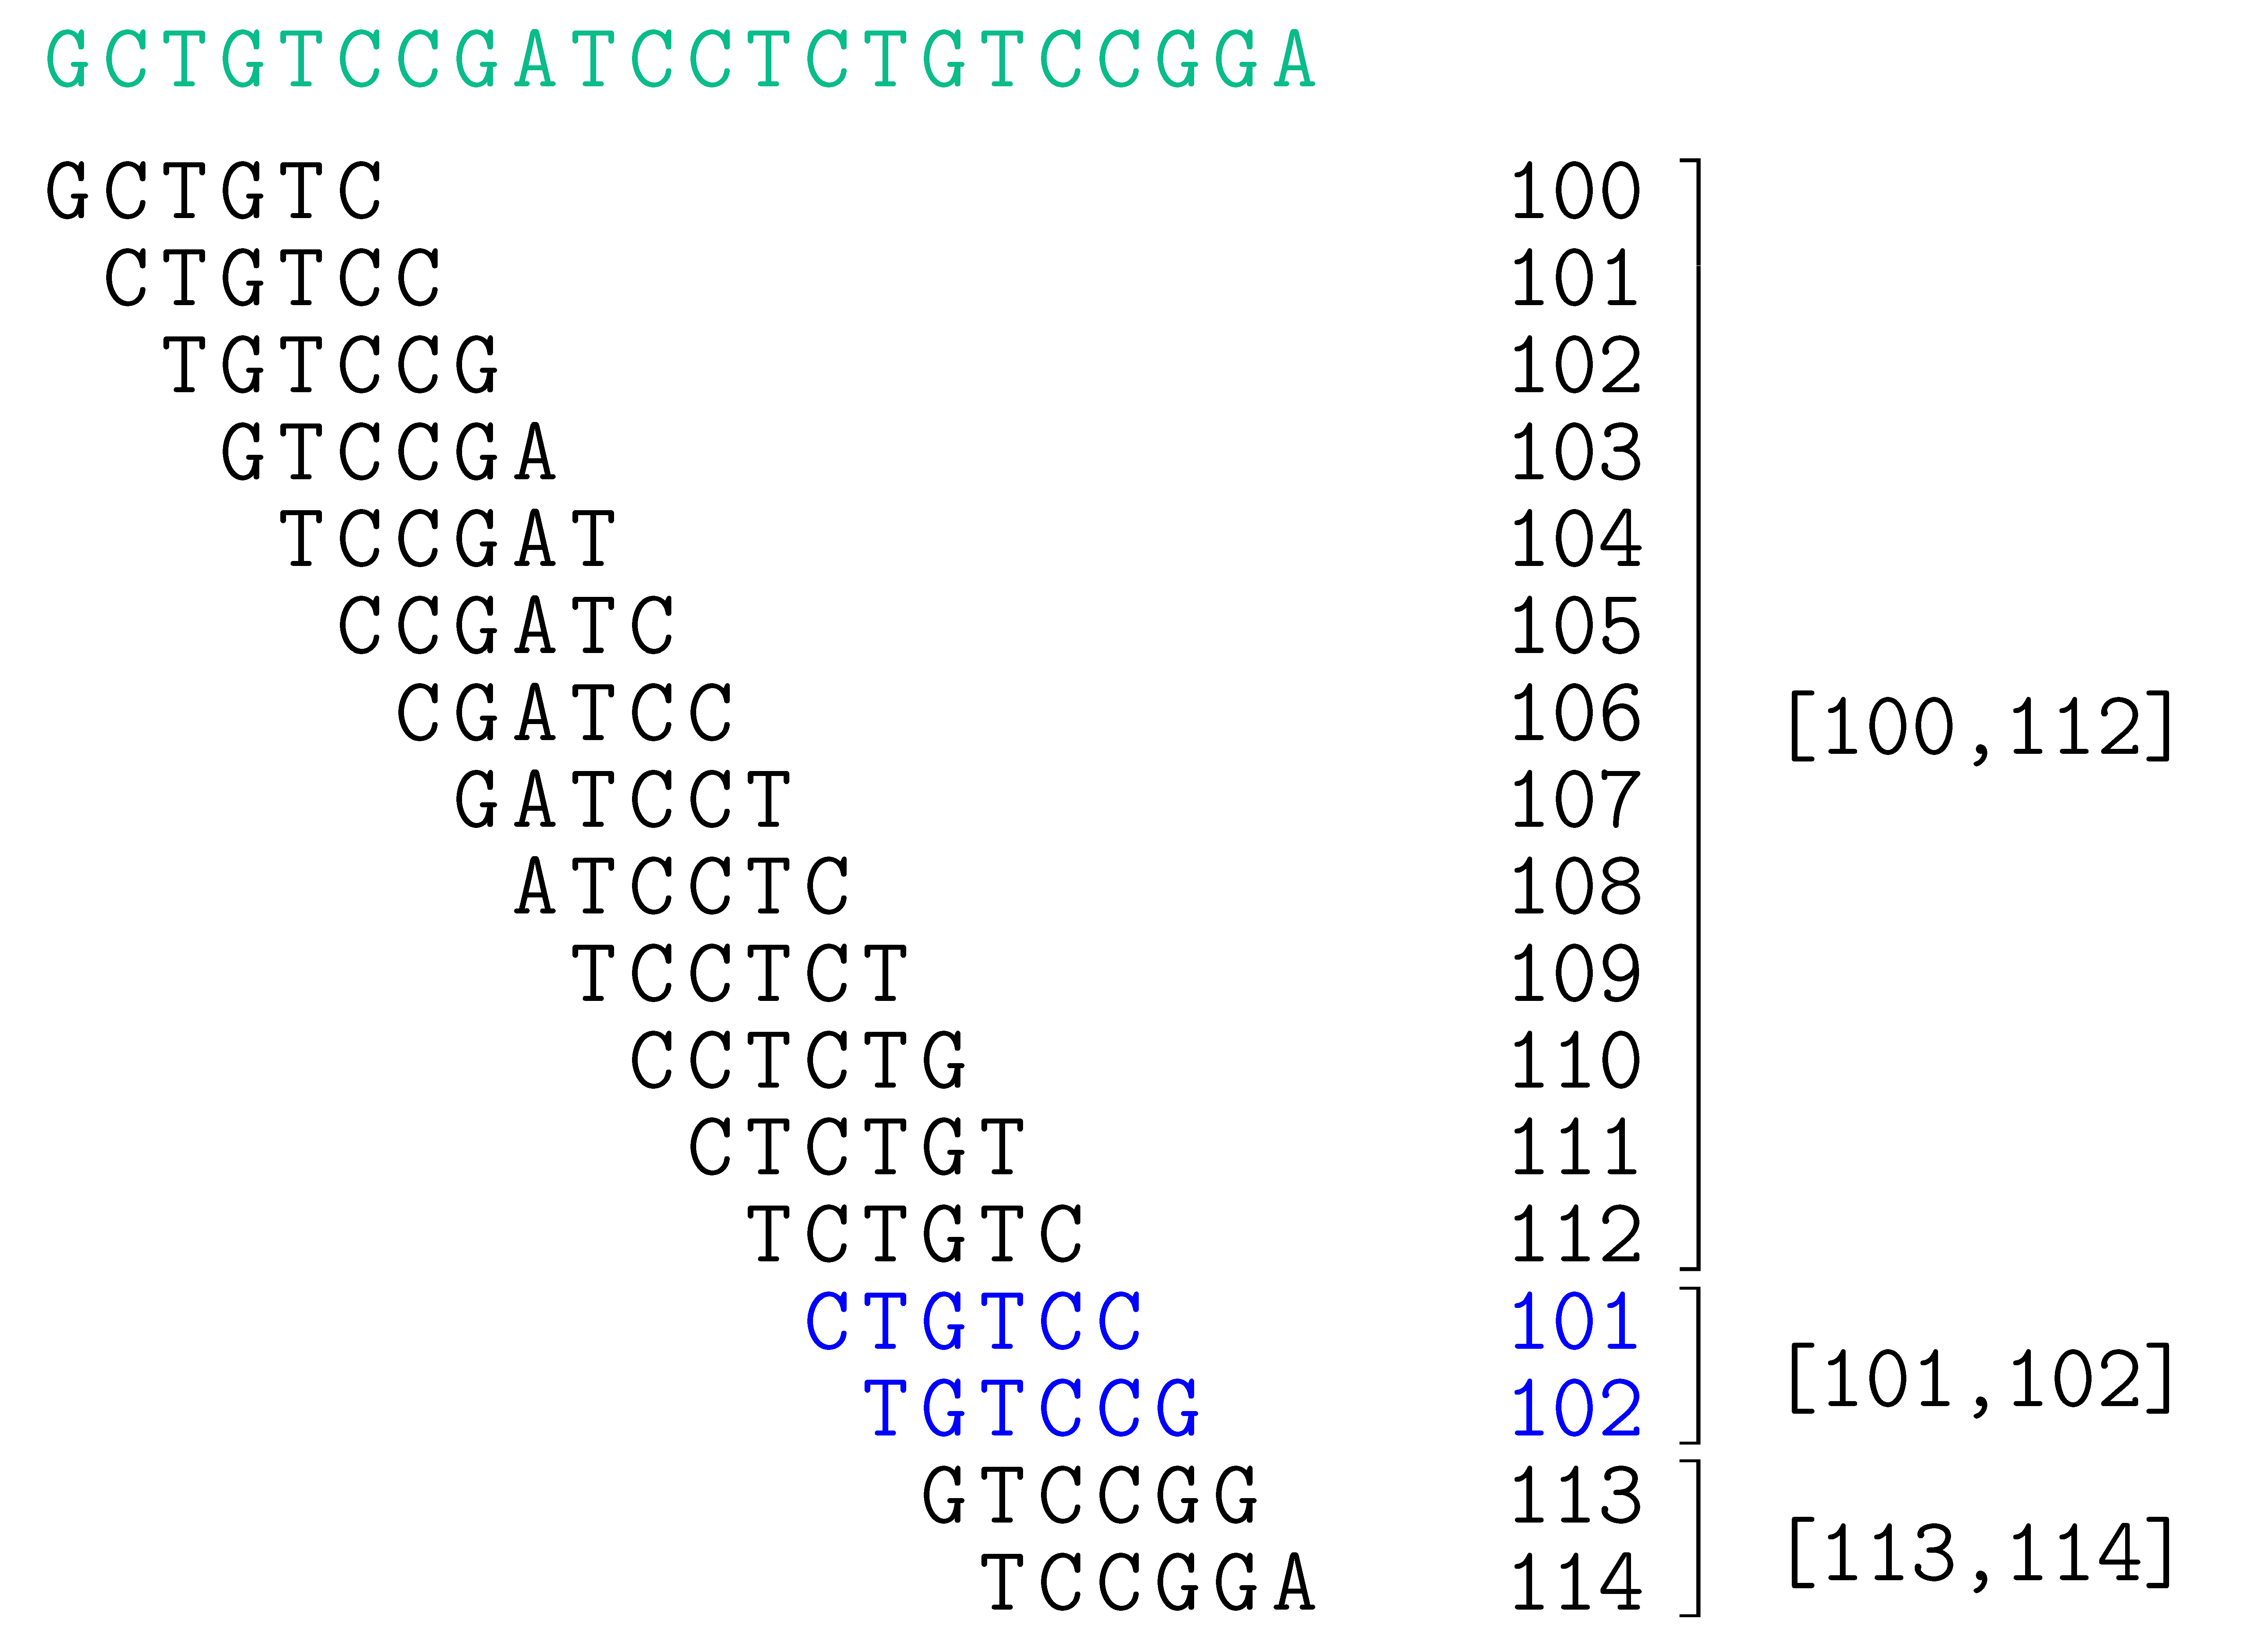
\includegraphics[width=0.6\textwidth]{capitoli/allpaths/numbering.png}
		\caption{Esempio di numerazione dei k-mer e traduzione della sequenza in intervalli. Posto $k=6$, vengono individuati tutti i k-mer presenti, ognuno dei quali viene numerato con un numero unico, riutilizzandolo nel caso di k-mer ripetuti. Usando gli intervalli, la sequenza iniziale viene quindi tradotta in $([100,112], [101, 102], [113, 114])$.}
		\label{fig:allpathsnumbering}
	\end{figure}
	
	\paragraph{Formazione degli unipath}
	Tutti i numeri degli intervalli trovati nei k-mer path vengono scanditi. L'obiettivo per ogni numero è trovare il più lungo intervallo senza interruzioni che lo contenga. Si cercano nel database tutti gli intervalli che contengono quel numero, e si sceglie l'intervallo continuo più lungo, che diventa un \textit{unipath interval}. Il processo è ripetuto per tutti i k-mer che non sono stati ancora inclusi in un unipath interval. 
	
	Per ogni unipath interval viene preso il primo numero di k-mer; esso viene cercato nel database e viene determinato, se presente, un suo possibile predecessore. Se ne esiste esattamente uno, l'unipath interval del primo numero viene collegato all'intervallo alla sua sinistra. Procedendo iterativamente, viene formato un unipath, che consiste quindi in un gruppo di k-mer contigui. 
	
	\paragraph{Isolamento dei seed unipath}
	Tra gli unipath creati, è possibile isolare dei \textit{seed unipath}, attorno ai quali poi eseguire l'assembly. Preso l'insieme di tutti gli unipath, iterativamente si rimuovono alcuni di essi; preso un certo unipath $u$, si isolano quelli adiacenti a destra e a sinistra rispetto a $u$. Tra i due vicini di $u$ viene dedotta la distanza; se essa è minore di una certa soglia, $u$ può essere rimosso dall'insieme. Si procede in questo modo per tutti gli unipath presenti, finché continua a essere possibile la rimozione. Gli unipath rimasti costituiranno un seed unipath.
	
	\paragraph{Assembly locale e globale}
	Attorno ai seed unipath viene quindi assemblato il vicinato (\textit{neighborhood}), cioè le regioni di 10 kb che precedono e seguono il seme. Per farlo, vengono creati due gruppi di sequenze, il primo (\textit{primary read cloud}) contenente letture la cui posizione reale è vicina al seme, mentre il secondo (\textit{secondary read cloud}) contiene brevi frammenti la cui sequenza può essere assemblata con le letture del primo gruppo. Il vicinato dei semi viene quindi assemblato utilizzando i due gruppi di letture, formando un \textit{sequence graph} dell'assembly locale, cioè attorno al seed unipath corrispondente.
	
	I vari assembly locali vengono fatti in parallelo, e sono poi uniti per formare un sequence graph unico, relativo cioè all'assembly globale.
	
	
	\subsection{Gestione di genomi di grandi dimensioni}
	I predecessori di ALLPATHS-LG ottengono risultati promettenti solo per genomi di piccole dimensioni. Per gestire genomi di dimensioni più grandi, come quelli di mammiferi, sono state fatte delle modifiche notevoli \cite{gnerre2011high}.

	Il programma cerca di comprimere le ripetizioni in modo da favorirne l'allineamento. Se una sequenza ripetitiva è presente in due letture separate, il programma utilizza un'altra coppia di shotgun per poter allineare le prime due (\textit{gap filling}). Le letture vengono unite se un'altra coppia fornisce una sovrapposizione, e viceversa. Il metodo può essere utilizzato anche se sono presenti mutazioni \gls{snp}, che forniscono più soluzioni di assemblamento. La figura~\vref{fig:allpathsfilling} tratta da \cite{gnerre2011high} mostra come avviene la gestione delle sequenze ripetitive nei due diversi casi.

	\begin{figure}
		\centering
		\subfloat[][\emph{L'allineamento della coppia di letture in nero è possibile usando un'altra coppia di letture, raffigurate in rosso.}]
		{
\includegraphics[width=0.6\textwidth]{capitoli/allpaths/filling1.png}} \\
		\subfloat[][\emph{Le due coppie di letture in rosso potrebbero allineare la coppia di letture in nero, ma presentano un SNP. Vengono quindi mantenute entrambe, fornendo due diverse soluzioni possibili.}]
		{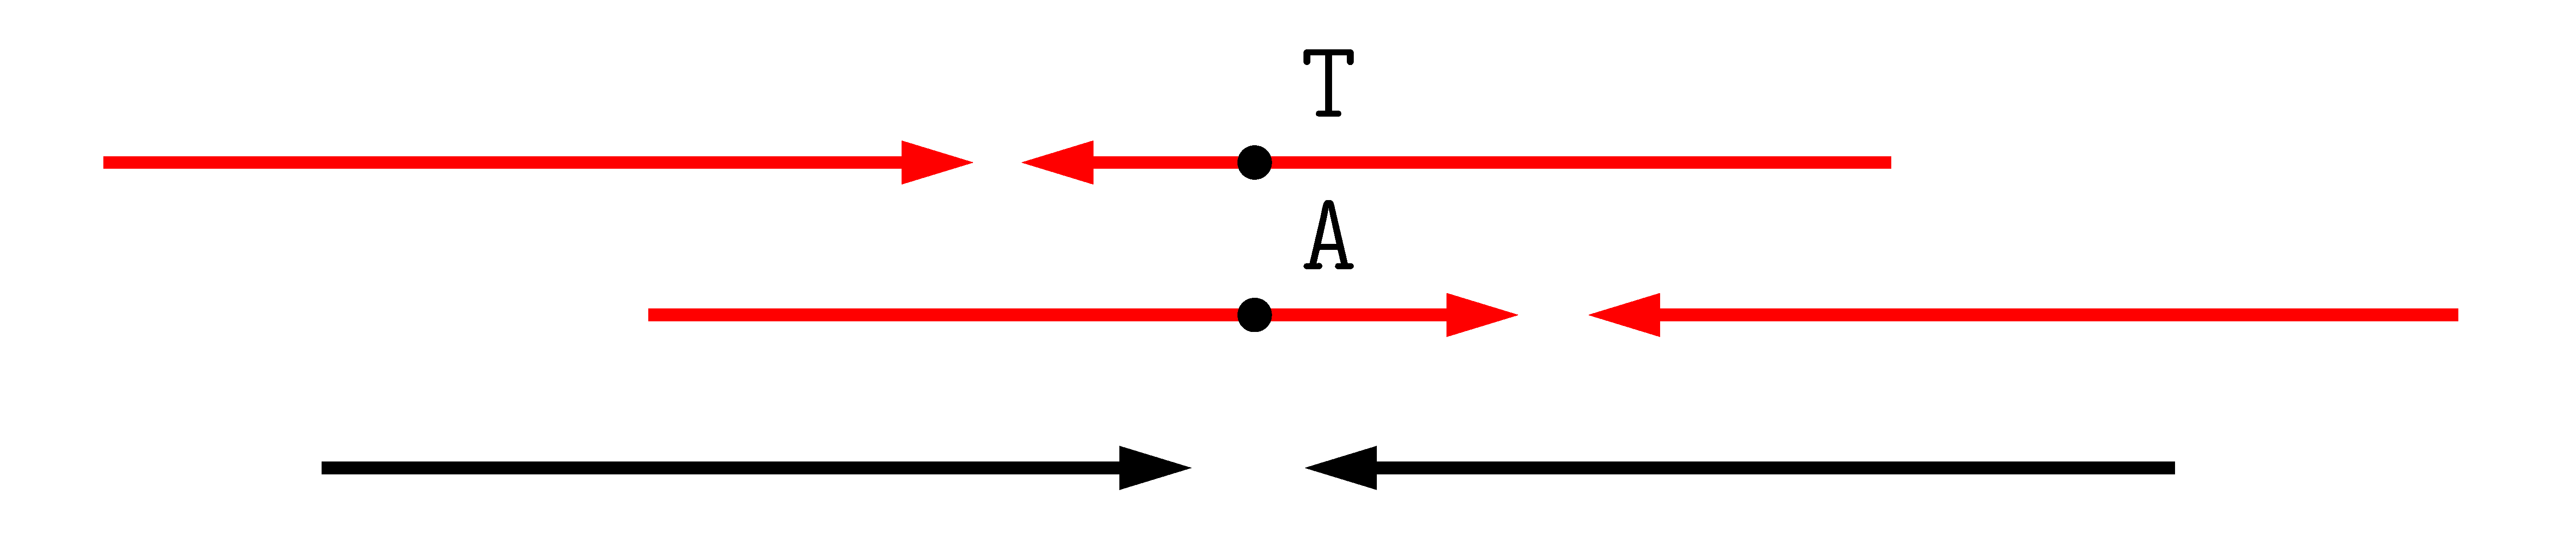
\includegraphics[width=0.6\textwidth]{capitoli/allpaths/filling2.png}} 
		\caption{Esempi grafici del processo di gap filling.}
		\label{fig:allpathsfilling}
	\end{figure}
	
	La nuova versione del programma inoltre migliora la correzione degli errori di lettura: dato un k-mer, vengono analizzate tutte le letture che lo contengono; nel caso una singola lettura differisca dalla maggior parte delle altre, essa viene corretta se non ci sono voti in conflitto, altrimenti non viene modificata.
	
	Ulteriori miglioramenti sono fatti anche per la gestione di sequenze a bassa copertura: dato che in questi casi la sovrapposizione tra letture può essere breve, in tali zone è preferibile utilizzare k-mer di dimensioni minori cioè scegliere un valore di $k$ più basso. Il programma permette di utilizzare un valore di $k>15$, ma solo nelle regioni che sarebbero assegnate a uno spazio vuoto tra altre due sequenze. 
	
	\subsection{Stima della dimensione del genoma}
	TODO
	
	
	
	
	
	
	
	
\end{document}